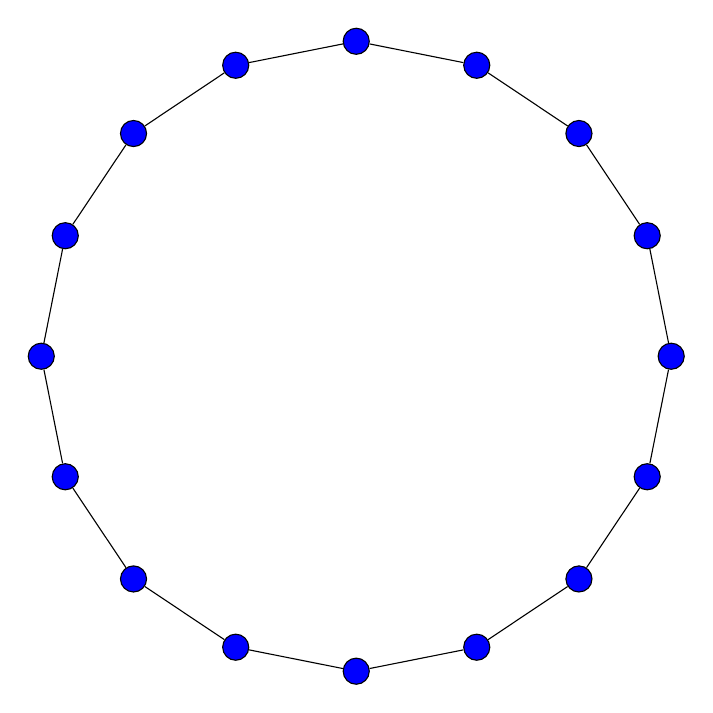
\begin{tikzpicture}
  \def\nodes{16}
  \def\radius{4}
  \foreach \i in {1,...,\nodes} {
      \node[draw, fill=blue, circle, minimum size=6pt] (v\i) 
      at ({\i*360/\nodes}: \radius) {};
  }

  \foreach \i in {1,...,\nodes} {
      \pgfmathtruncatemacro{\j}{mod(\i, \nodes) + 1}
      \draw (v\i) -- (v\j);
  }
\end{tikzpicture}